\documentclass{article}
\usepackage[
    letterpaper,
    top=1in,
    bottom=1in,
    inner=0.75in,
    outer=0.75in,
    % margin=1in,
]{geometry}

%%%% Page Header and Foot %%%%
\usepackage{fancyhdr}
\fancypagestyle{plain}{
\fancyhf{}
\fancyhead[L]{Rutgers University}
\fancyhead[C]{16:332:545 Digital Communications}
\fancyhead[R]{Spring 2024}
\fancyfoot[L]{}
\fancyfoot[C]{\thepage}
\fancyfoot[R]{}
}
\pagestyle{plain}

%%%% Load Format %%%%
%%%% Page Margin %%%%
\RequirePackage{geometry}

%%%% Page Header and Foot %%%%
\RequirePackage{fancyhdr}
\pagestyle{fancyplain}
\lhead{\lefthead}
\chead{\centerhead}
\rhead{\righthead}
\lfoot{\leftbottom}
\cfoot{\centerbottom}
\rfoot{\rightbottom}

%%%% Additional Packages to Load %%%%
%%%% Main Font
\RequirePackage{lmodern} %Computer Modern, but with many more glyphs
\RequirePackage{microtype} %Better Font Rendering
\RequirePackage{libertinus} %Very popular math font
\RequirePackage[T1]{fontenc} %Better Printing Font
\RequirePackage[utf8]{inputenc} %enable utf8 encoding
\RequirePackage[english]{babel} %English Language

%%%% Math Env
\RequirePackage{amsfonts,amsmath,amssymb} %Math Font Packages
\RequirePackage{mathtools} %Better Math Environments
\RequirePackage{mleftright}  %Fixes some annoying spacing issues
\RequirePackage{bm} %Boldface math, load after other math font packages

%%%% Beautiful Stuff
\RequirePackage{graphicx} %Better Graphics
\RequirePackage[export]{adjustbox} %Better Graphics
\RequirePackage[dvipsnames,svgnames]{xcolor} %Must load before tcolorbox
\RequirePackage[breakable]{tcolorbox} %Customized Box
\tcbuselibrary{skins}
\RequirePackage{transparent} 

%%%% Table and List 
\RequirePackage{tabularx} %Better Table
\RequirePackage{multirow}
\RequirePackage{colortbl}
\RequirePackage{array}

%%%% Theorems etc (also  problems)
\RequirePackage[shortlabels]{enumitem} %Better List
\RequirePackage{hyperref, cleveref} %Fantastic crossrefer
\RequirePackage{amsthm, thmtools} %Better Theorems
\RequirePackage{thm-restate} %Better Theorems

%%%% Code Packages
\RequirePackage{algorithm2e} % Package to create pseudo-code
\RequirePackage{listings} % Package to insert code
% \RequirePackage{keyval}

%%%% Display Packages
\RequirePackage[document]{ragged2e} % Package to justify text
\RequirePackage{csquotes} % Package to facilities quotations
\RequirePackage{multicol} % Package to use multicols

%%%% Other Packages
\RequirePackage{calc}
\RequirePackage{rotating}
\RequirePackage{pgf, tikz}
\RequirePackage{epstopdf}
\RequirePackage[backend=biber, style=numeric, sorting=none]{biblatex}

%%%% A box fill the rest of the page
\newtcolorbox{stretchbox}[1][]{
    height fill,
    sharp corners,
    colback=white,
    % colframe=yellow!50!black,
    #1
    }

%%%% Box Environment
\newtcolorbox{prob}[1]{
% Set box style
    sidebyside,
    sidebyside align=top,
% Dimensions and layout
    width=\textwidth,
    toptitle=2.5pt,
    bottomtitle=2.5pt,
    righthand width=0.20\textwidth,
% Coloring
    colbacktitle=white,
    coltitle=black,
    colback=white,
    colframe=black,
% Title formatting
    title={
        #1 \hfill Grade:\hspace*{0.15\textwidth}
    },
    fonttitle=\large\bfseries
}

%%%% Problem Environment 
\newenvironment{problem}[1]{
    \begin{prob}{#1}
}
{
    \tcblower
    \centering
    \textit{\scriptsize\bfseries Faculty Comments}
    \end{prob}
}

%%%% Draw a line
\newcommand{\myrule}{\rule{1.5in}{0.1mm}}
%%%% delimiters
\DeclarePairedDelimiter\parens{\lparen}{\rparen}
\DeclarePairedDelimiter\bracks{\lbrack}{\rbrack}
\DeclarePairedDelimiter\braces{\lbrace}{\rbrace}
\DeclarePairedDelimiter\abs{\lvert}{\rvert}
\DeclarePairedDelimiter\norm{\lVert}{\rVert}
\DeclarePairedDelimiter\angles{\langle}{\rangle}
\DeclarePairedDelimiter\ceil{\lceil}{\rceil}
\DeclarePairedDelimiter\floor{\lfloor}{\rfloor}

%%%% math operators naming
\DeclareMathOperator*{\argmax}{\textnormal{argmax}}
\DeclareMathOperator*{\argmin}{\textnormal{argmin}}
\DeclareMathOperator{\tr}{\textnormal{tr}}
\DeclareMathOperator{\eig}{\textnormal{eig}}
\DeclareMathOperator{\sgn}{\textnormal{sgn}}
% \let\det\relax % "Undefine" \det
% \DeclareMathOperator{\det}{\textnormal{det}} % already defined in mathtools
\DeclareMathOperator{\diag}{\textnormal{diag}}
\DeclareMathOperator{\rank}{\textnormal{rank}}
\DeclareMathOperator{\Vol}{\textnormal{Vol}}   % volume
\DeclareMathOperator{\Surf}{\textnormal{Surf}} % surface area

%%%% Transforms! -- requires mathtools package
\newcommand*{\LapTrans}{\xleftrightarrow{\mathcal{Z}}}
\newcommand*{\ZTrans}{\xleftrightarrow{\mathcal{L}}}
\newcommand*{\CTFS}{\xleftrightarrow{\textnormal{CTFS}}}
\newcommand*{\CTFT}{\xleftrightarrow{\textnormal{CTFT}}}
\newcommand*{\DTFS}{\xleftrightarrow{\textnormal{DTFS}}}
\newcommand*{\DTFT}{\xleftrightarrow{\textnormal{DTFT}}}

%%%% vector font
\let\oldvec\vec
\renewcommand*{\vec}[1]{\mathbf{#1}}
% \newcommand*{\trn}{\!^{\!\intercal}}
\newcommand*{\trn}{\!^{\mathsf{T}}}
% \newcommand*{\coj}{\!^{\dag}} % Text Mode Symbol, Should not be used
% \newcommand*{\coj}{\!^{\dagger}}
\newcommand*{\coj}{\!^{\mathsf{H}}}
\newcommand*{\inv}{^{-1}}

%%%% number systems
\DeclareMathOperator{\R}{\mathbb{R}}
\DeclareMathOperator{\C}{\mathbb{C}}
\DeclareMathOperator{\N}{\mathbb{N}}
\DeclareMathOperator{\Z}{\mathbb{Z}}
\DeclareMathOperator{\F}{\mathbb{F}}
\DeclareMathOperator{\Q}{\mathbb{Q}}

%%%% STATISTICS AND PROBABILITY
\newcommand*{\Var}{\mathop{\textnormal{Var}}}
\newcommand*{\Cov}{\mathop{\textnormal{Cov}}}
\newcommand*{\Corr}{\mathop{\textnormal{Corr}}}
\newcommand*{\MSE}{\mathop{\textnormal{MSE}}}
\newcommand*{\MSD}{\mathop{\textnormal{MSD}}}
\newcommand*{\NSD}{\mathop{\textnormal{NSD}}}

\newcommand*{\E}[1]{\mathbb{E}\bracks*{#1}}
\newcommand*{\condE}[2]{\mathbb{E}\bracks*{#1 \mid #2}}
\renewcommand*{\P}[1]{\mathbb{P}\parens*{#1}}
\newcommand*{\condP}[2]{\mathbb{P}\parens*{#1 \mid #2}}

\DeclareMathOperator{\Bern}{\mathsf{Bern}}
\DeclareMathOperator{\Unif}{\mathsf{Unif}}
\DeclareMathOperator{\Expv}{\mathsf{Exp}}
\DeclareMathOperator{\Poi}{\mathsf{Poi}}
\DeclareMathOperator{\Gamv}{\mathsf{Gamma}}
\DeclareMathOperator{\Dirv}{\mathsf{Dir}}
\DeclareMathOperator{\Mult}{\mathsf{Mult}}
\DeclareMathOperator{\Beta}{\mathsf{Beta}}
\DeclareMathOperator{\Geomv}{\mathsf{Geom}}
\DeclareMathOperator{\Binomv}{\mathsf{Binom}}
\DeclareMathOperator{\NegBinomv}{\mathsf{NB}}
\DeclareMathOperator{\Lap}{\mathsf{Lap}}
\DeclareMathOperator{\Gaus}{\mathsf{N}}
\DeclareMathOperator{\Weibull}{\mathsf{Weibull}}


\DeclareMathOperator{\iidsim}{\stackrel{\textnormal{i.i.d.}}{\sim}}
\DeclareMathOperator{\diff}{\mathop{}\!\textnormal{d}}

%%%% Special norms and linear algebra stuff
\newcommand*{\subgnorm}[1]{\norm*{#1}_{\psi_2}}
\newcommand*{\subexpnorm}[1]{\norm*{#1}_{\psi_1}}
\newcommand*{\frobnorm}[1]{\norm*{#1}_{\textnormal{F}}}
\newcommand*{\opnorm}[1]{\norm*{#1}_{\textnormal{op}}}
\newcommand*{\Lipnorm}[1]{\norm*{#1}_{\textnormal{Lip}}}

%%%%
\newcommand*{\set}[1]{\braces*{\,#1\,}}
\newcommand*{\ie}{\textnormal{i.e.\ }}
\newcommand*{\eg}{\textnormal{e.g.\ }}
\newcommand*{\etc}{\textnormal{etc.\ }}
\newcommand*{\iid}{\textnormal{i.i.d.\ }}
\allowdisplaybreaks

%%%% Theorem Style %%%%
\declaretheorem[numbered=no, style=plain]{axiom, lemma}
\declaretheorem[numberwithin=section,style=definition]{definition}
\declaretheorem[sibling=definition]{theorem, corollary, proposition, conjecture}
\declaretheorem[numbered=no,style=remark]{remark, claim}

%%%% Document Information %%%%
\title{Project on OFDM Communications}
\author{Kailong Wang}
\date{\today}

\addbibresource{bib.bib}
% \graphicspath{ {../MyOFDM_1/} }
% \epstopdfsetup{outdir=./}

%%%% Start Document %%%%
\begin{document}
\maketitle

\begin{abstract}
    Orthogonal Frequency Division Multiplexing (OFDM)~\cite{5307460} is a popular modulation scheme in modern wireless communications. It achieves high symbol rates while being robust to frequency-selective fading and intersymbol interference. This project discusses the OFDM technique and evaluates its performance with simulations. The project consists of following parts as required:
    \begin{enumerate}[(i)]
        \item A description of the OFDM modulation and demodulation process.
        \item A discussion of the advantages and disadvantages of OFDM technique.
        \item The usage of pilot symbols for channel estimation in OFDM system.
        \item Numerical results to evaluates the OFDM scheme.
    \end{enumerate}
\end{abstract}

\section{Modulation and Demodulation}
\label{sec:modulation}
In designing the digital communication system, the complex physical environment (channel) limits the communication capacity and challenges the robustness of the system. A short duration, high symbol rate signal is not robust to multipath environment, which is the common situation, while a long duration , low symbol rate signal cannot satisfy modern communication demand. Thanks to the Uncertainty Principle~\cite{BibEntry2021Dec}, which states the long duration signal has a narrow bandwidth, if the total bandwidth can be used to transmit multiple narrow bandwidth signals simultaneously, the communication capacity can be improved without sacrificing the robustness. The Orthogonal Frequency Division Multiplexing (OFDM) technique is designed to achieve this goal.
In this section we describe the modulation and demodulation process of Orthogonal Frequency Division Multiplexing (OFDM) system.

The Modulation of the OFDM system can be summarized as follows:
\begin{enumerate}[(i)]
    \item A message is encoded into a bit stream with length $N\log_2M$, where $N$ is the number of narrowband subcarriers and $M$ is the modulation order.
    \item The bit stream is mapped into $N$ complex information symbols using a modulation scheme such as M-PSK, M-QAM, \etc. The resulting symbol sequence can be expressed as $[X_{0}, X_{1}, \ldots, X_{N-1}]$.
    \item This sequence passes through a serial-to-parallel converter to form a block as $X = [[X_{0}], [X_{1}], \ldots, [X_{N-1}]]$.
    \item Using the Inverse Fast Fourier Transform (IFFT), the block $X$ is converted into time domain $x = [[x_0], [x_1], \allowbreak \ldots, [x_{N-1}]]$, where
    \begin{equation}
        \label{eq:IFFT}
        x_n = \sum_{i=0}^{N-1}X_i e^{j2\pi\frac{i}{N}n} \qquad n=0,1,\ldots,N-1.
    \end{equation}
    \item The cyclic prefix is added by copying the last $L$ samples of $x$ and appending them to the beginning of $x$, where $L$ is the length of the cyclic prefix. This block passes through a parallel-to-serial converter, and then converts the digital samples, $x[n] = [x_{N-L}, x_{N-L+1}, \ldots, x_{N-1}, x_0, x_1, \ldots, x_{N-1}]$, to an analog baseband signal $x(t)$ by a Digital to Analog Converter (DAC).
\end{enumerate}

The signal $x(t)$ is upconverted to the carrier frequency $f_c$ and transmitted over the channel. Suppose the channel is Linear Time Invariant (LTI), it would have the effect as a filter which can be characterized by Finite Impulse Response (FIR) $h(t)$. The channel also corrupts the signal with Additive White Gaussian Noise (AWGN) $w(t)$. The received signal is downconverted to baseband, passes through a low pass filter to remove the high frequency component (noise), and sampled by the Analog to Digital Converter (ADC), resulting digital samples $y[n] = x[n] \circledast h[n] +  w[n]$, which can be expressed as $[y_{N-L}, y_{N-L+1}, \ldots, y_{N-1}, y_0, y_1, \ldots, y_{N-1}]$. Operator $\circledast$ is convolution.

The Demodulation of the OFDM system can be summarized as follows:
\begin{enumerate}[(i)]
    \item The digital samples $y[n]$ contains $N+L$ elements. The cyclic prefix is removed by discarding the first $L$ elements. After a serial-to-parallel converter, the resulting block is $y = [[y_0], [y_1], \ldots, [y_{N-1}]]$.
    \item Using the Fast Fourier Transform (FFT), the block $y$ is converted into frequency domain $Y = [[Y_{0}], [Y_{1}], \ldots, [Y_{N-1}]]$, where
    \begin{equation}
        Y_i = \sum_{n=0}^{N-1}y_n e^{-j2\pi i\frac{n}{N}} \qquad i=0,1,\ldots,N-1.
    \end{equation}
    \item Each element in the block is a complex information symbol. After a parallel-to-serial converter, the symbol sequence can be expressed as $[Y_{0}, Y_{1}, \ldots, Y_{N-1}]$.
    \item These symbols are demodulated by the corresponding $M$-ordered demodulation scheme to recover the original bit stream with length $N\log_2M$.
    \item The recovered bit stream is decoded to the original message.
\end{enumerate}

\section{Advantages and Disadvantages}
The OFDM modulation and demodulation look trivial but some non-trivial features are hidden in the process and worth to mention explicitly.

\subsection{Orthogonality, Symbol Rate and Guard Interval/Cyclic Prefix}
To guarantee each narrowband symbol would not interfere others, the subcarriers in OFDM are designed to be orthogonal to each other. This means that the cross-correlation between any two subcarriers is zero. This property also guarantee the maximum number of subcarriers to be transmitted simultaneously. To achieve this, the subcarriers are spaced at $\triangle f=\frac{1}{T}$ Hz, where $T$ is the OFDM symbol duration. This can be proved as follows.
\begin{proof}
    Let $f_i=i\triangle f$ and $f_j=j\triangle f$ be the frequencies of two subcarriers, the cross-correlation between them is
    \begin{align*}
        \ip{e^{j2\pi f_i t}, e^{j2\pi f_j t}}
        &= \frac{1}{T}\int_{0}^{T} (e^{j2\pi f_i t}) (e^{j2\pi f_j t})^* \diff t \\
        &= \frac{1}{T}\int_{0}^{T} e^{j2\pi (f_i - f_j) t} \diff t \\
        &= \frac{1}{T}\int_{0}^{T} e^{j2\pi (i - j)\triangle f t} \diff t \\
        &= \frac{\sin(\pi T(i-j)\triangle f)}{\pi T(i-j)\triangle f}e^{j\pi T(i-j)\triangle f}. \\
        \Re[\ip{e^{j2\pi f_i t}, e^{j2\pi f_j t}}]
        &= \frac{\sin(\pi T(i-j)\triangle f)}{\pi T(i-j)\triangle f}\cos(j\pi T(i-j)\triangle f) \\
        &= \frac{\sin(2\pi T(i-j)\triangle f)}{2\pi T(i-j)\triangle f} \\
        &= \sinc(2T(i-j)\triangle f).
    \end{align*}
    To make the cross-correlation zero, we need to have $2T(i-j)\triangle f = k$ for some integer $k$ when $i\neq j$. This implies that $T\cdot\triangle f=1$.
\end{proof}
The~\cref{fig:orthogonality} shows the cross-correlation between two subcarriers with different spacing. The cross-correlation is zero when the subcarriers are spaced at $\triangle f=\frac{1}{T}$ Hz.

With the orthogonality of the subcarriers, the OFDM is able to transmit $N$ information symbols (\ie QAM, PSK, \etc) in parallel in each duration $T$, resulting in high OFDM symbol rate, $R_s=\frac{N}{T}$ symbols per second. And hence the duration $T$ can be longer than other modulation schemes when the same amount of information is transmitted.
The longer duration $T$ gives OFDM rooms to add the guard interval in between each OFDM symbol. By setting the length of the guard interval to be longer than the channel delay spread, the OFDM system can combat the intersymbol interference caused by the multipath delay. The guard interval is usually implemented as the cyclic prefix as described above.

\begin{figure}[!htbp]
    \centering
    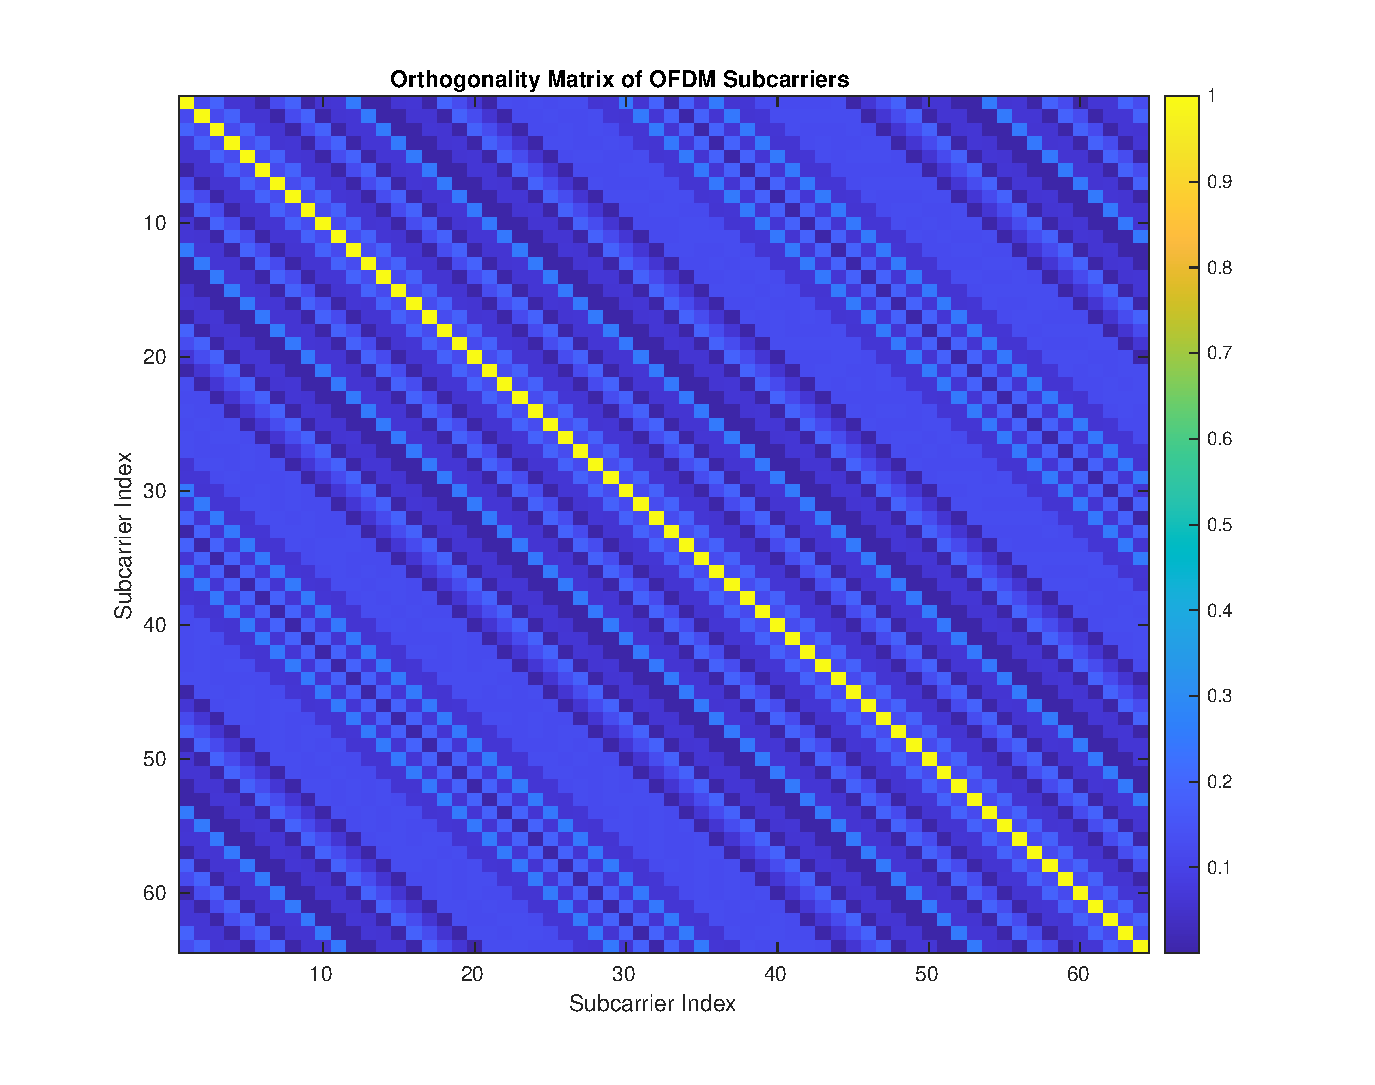
\includegraphics[width=\linewidth]{Orthogonality.eps}
    \caption{Subcarriers = $64$, CP = $16$, SNR = $20$ dB.}
    \label{fig:orthogonality}
\end{figure}

\subsection{Circular Convolution, Circulant Matrices and Intersymbol Interference (ISI)}
The cyclic prefix leads to circular convolution between the channel impulse response and the transmitted signal. We show this mathematical fact and its properties as follows. The content is based on~\cite{91291216} and is modified with the content in~\cite{2024Apr}.

We use the same notation as defined above. We first show that the cyclic prefix of $y[n]$ can be safely discard. Suppose the channel delay spread is the same as the length of the cyclic prefix $L$. Then the received signal $y[n]$ can be written as
\begin{equation}
    \label{eq:circ_conv}
    \begin{bmatrix}
        y_{N-1} \\ y_{N-2} \\ \vdots \\ y_1 \\ y_0
    \end{bmatrix}
    =
    \begin{bmatrix}
        h_0 & h_1 & \cdots & h_{L} & 0 & \cdots & 0 & 0 & \cdots & 0 \\
        0 & h_0 & \cdots & h_{L-1} & h_{L} & \cdots & 0 & 0 & \cdots & 0 \\
        \vdots & \vdots & \ddots & \vdots & \vdots & \ddots & \vdots & \vdots & \ddots & \vdots \\
        0 & 0 & \cdots & 0 & 0 & \cdots & h_0 & h_1 & \cdots & 0 \\
        0 & 0 & \cdots & 0 & 0 & \cdots & 0 & h_0 & \cdots & h_{L}
    \end{bmatrix}
    \begin{bmatrix}
        x_{N-1} \\ x_{N-2} \\ \vdots \\ x_1 \\ x_0 \\ x_{N-1} \\ \vdots \\ x_{N-L}
    \end{bmatrix}
    +
    \begin{bmatrix}
        w_{N-1} \\ w_{N-2} \\ \vdots \\ w_1 \\ w_0
    \end{bmatrix}
\end{equation}
where $h_l$ is the channel impulse response of the $l$-th channel. The above matrices show that discarding the cyclic prefix at the receiver does not affect the received signal $y[n]$. It is also clear that the above representation will remain valid as long as the channel delay spread is less than the length of the cyclic prefix, since setting the $h_l$ to be zero will not affect the above representation. But longer delay spread will violate that. This mathematical fact also tells that the ISI of OFDM symbols is eliminated by discarding the cyclic prefix in the OFDM system.

With some algebra, the above representation can be written as
\begin{equation}
    \label{eq:circ_conv2}
    \begin{bmatrix}
        y_{N-1} \\ y_{N-2} \\ \vdots \\ y_1 \\ y_0
    \end{bmatrix}
    =
    \begin{bmatrix}
        h_0 & h_1 & \cdots & h_{L-2} & h_{L-1} & h_{L} & 0 & \cdots & 0 & 0 \\
        0 & h_0 & \cdots & h_{L-3} & h_{L-2} & h_{L-1} & h_{L} & \cdots & 0 & 0 \\
        \vdots & \vdots & \ddots & \vdots & \vdots & \vdots & \vdots & \ddots & \vdots & \vdots \\
        h_2 & h_3 & \cdots & h_{L} & 0 & 0 & 0 & \cdots & h_0 & h_1 \\
        h_1 & h_2 & \cdots & h_{L-1} & h_{L} & 0 & 0 & \cdots & 0 & h_0
    \end{bmatrix}
    \begin{bmatrix}
        x_{N-1} \\ x_{N-2} \\ \vdots \\ x_1 \\ x_0
    \end{bmatrix}
    +
    \begin{bmatrix}
        w_{N-1} \\ w_{N-2} \\ \vdots \\ w_1 \\ w_0
    \end{bmatrix}
\end{equation}
\begin{equation}
    \mtx{y} = \mtx{H}\mtx{x} + \mtx{w}.
\end{equation}
The~\cref{eq:circ_conv} is the actual signal at the receiver while the~\cref{eq:circ_conv2} is an analytical equivalent, which is circular convolution. The matrix $\mtx{H}$ is an $N\times N$ matrix induced from an $N\times(N+L)$ matrix and is a special type of matrix called circulant matrix. Hence, the $\mtx{H}$ can be expressed as
\begin{equation}
    \label{eq:circ_mat}
    \mtx{H} = h_0\mtx{I}+h_1\mtx{P}+h_2\mtx{P}^2+\cdots+h_L\mtx{P}^L,
\end{equation}
where $\mtx{P}$ is an $N\times N$ permutation matrix
\begin{equation}
    \mtx{P} = \begin{bmatrix}
        0 & 1 & 0 & \cdots & 0 & 0 \\
        0 & 0 & 1 & \cdots & 0 & 0 \\
        \vdots & \vdots & \vdots & \ddots & \vdots & \vdots \\
        0 & 0 & 0 & \cdots & 0 & 1 \\
        1 & 0 & 0 & \cdots & 0 & 0
    \end{bmatrix}.
\end{equation}

The~\cref{eq:circ_mat} tells us the eigenvectors of $\mtx{P}$ is the eigenvectors of $\mtx{H}$ since $\mtx{H}$ is a polynomial of $\mtx{P}$. It is also safe to hypothesis that the eigenvectors of $\mtx{H}$ are related to Fourier basis since $\mtx{H}$ is sort of periodic. Substituting~\cref{eq:circ_mat} in to $\det(\mtx{P}-\lambda\mtx{I})=0$ and evaluating different $N$, we can verify our hypothesis and find the orthonormal eigenvector matrix of $\mtx{H}$
\begin{equation}
    \mtx{F} = \frac{1}{\sqrt{N}}
    \begin{bmatrix}
        1 & 1 & 1 & \cdots & 1 \\
        1 & \omega & \omega^2 & \cdots & \omega^{N-1} \\
        1 & \omega^2 & \omega^4 & \cdots & \omega^{2(N-1)} \\
        \vdots & \vdots & \vdots & \ddots & \vdots \\
        1 & \omega^{N-1} & \omega^{2(N-1)} & \cdots & \omega^{(N-1)(N-1)}
    \end{bmatrix}
\end{equation}
\begin{equation}
    \omega = e^{-j2\pi\frac{1}{N}}.
\end{equation}

The matrix $\mtx{F}$ is the same as the discrete Fourier transform matrix. It provides the following properties:
\begin{enumerate*}[(i)]
    \item $\mtx{F}^{-1} = \mtx{F}\coj$;
    \item $\mtx{F}\coj\mtx{F}=\mtx{F}\mtx{F}\coj=\mtx{I}$;
    \item $\mtx{H}=\mtx{F}\Lambda\mtx{F}\coj=\mtx{F}\coj\Lambda\mtx{F}$ where $\Lambda$ is a diagonal matrix with the eigenvalues of $\mtx{H}$, \ie the frequency domain samples of the channel transfer function.
\end{enumerate*}
And leads to the following result of the demodulated OFDM symbol
\begin{equation}
    \label{eq:demod}
    \begin{aligned}
        \mtx{Y}
        &= \mtx{F}\mtx{y} \\
        &= \mtx{F}(\mtx{H}\mtx{x}+\mtx{w}) \\
        &= \mtx{F}(\mtx{F}\coj\Lambda\mtx{F}\mtx{F}\coj\mtx{X}+\mtx{w}) \\
        &= \Lambda\mtx{X} + \mtx{F}\mtx{w}.
    \end{aligned}
\end{equation}
The~\cref{eq:demod} states that the orthogonality of the subcarriers is preserved in the demodulated OFDM symbols.

\subsection{Equalization, Multipath Propagation and Frequency-Selective Fading}
The~\cref{eq:demod} reveals a simple equalization scheme for the OFDM system. The equalization can be done by multiplying the demodulated OFDM symbols by the inverse of the channel transfer function.
\begin{equation}
    \mtx{X} = \Lambda^{-1}\mtx{Y}.
\end{equation}
This is zero-forcing equalization. It is simple but doesn't work well when the channel transfer function has zeros or offsets at the frequency domain samples. In this case, the equalization will amplify the noise at the zeros. Besides, even when the offsets are not existed, the zero-forcing equalization doesn't benefit Signal to Noise Ratio (SNR). The minimum mean square error (MMSE) equalization, adaptive equalization, \etc are better approaches.

The existence of offsets in the channel transfer function is referred to frequency selective fading and caused by multipath propagation. This can be illustrated as follows. The channel impulse response can be expressed as
\begin{equation}
    h(t) = \sum_{l=0}^{L-1}h_l\delta(t-\tau_l),
\end{equation}
When $L=0$, the channel transfer function (the Fourier transform of $h_0$) is flat across whole bandwidth and the channel is said to be flat fading.
\begin{equation}
    \mtx{F}h_0(t-\tau_0) = h_0\cdot\mtx{F}\delta(t-\tau_0) = h_0\cdot e^{j2\pi f\tau_0}.
\end{equation}
When $L>0$, \aka multipath propagation, the channel transfer function becomes
\begin{equation}
    \begin{aligned}
        \mtx{F}h(t)
        &= \mtx{F}\sum_{l=0}^{L-1}h_l\delta(t-\tau_l) \\
        &= \sum_{l=0}^{L-1}h_l\mtx{F}\delta(t-\tau_l) \\
        &= \sum_{l=0}^{L-1}h_l e^{j2\pi f\tau_l}.
    \end{aligned}
\end{equation}
If $\abs{f\tau_{l_i}-f\tau_{l_j}}=\frac{4k-1}{2}$ for some integer $k$, then $\sgn(e^{j2\pi f\tau_{l_i}})=-\sgn(e^{j2\pi f\tau_{l_j}})$ and cause offsets in the channel transfer function~\cref{fig:ffading}. Frankly, the wideband signals suffer more from the frequency selective fading than narrowband signals because the wideband signals will have more frequency offsets across the bandwidth, while the narrowband signals can be considered flat because the bandwidth may locate in between the frequency offsets (\aka coherent bandwidth). The OFDM system is wideband but it is robust to frequency-selective fading because the subcarriers are spaced at $\triangle f=\frac{1}{T}$ Hz. This spacing is usually much smaller than the coherence bandwidth of the channel. Therefore, the channel can be considered flat over each subcarrier. This allows the OFDM system to use a simple equalizer (\ie zero-forcing) to combat the frequency-selective fading.

\begin{figure}[!htbp]
    \centering
    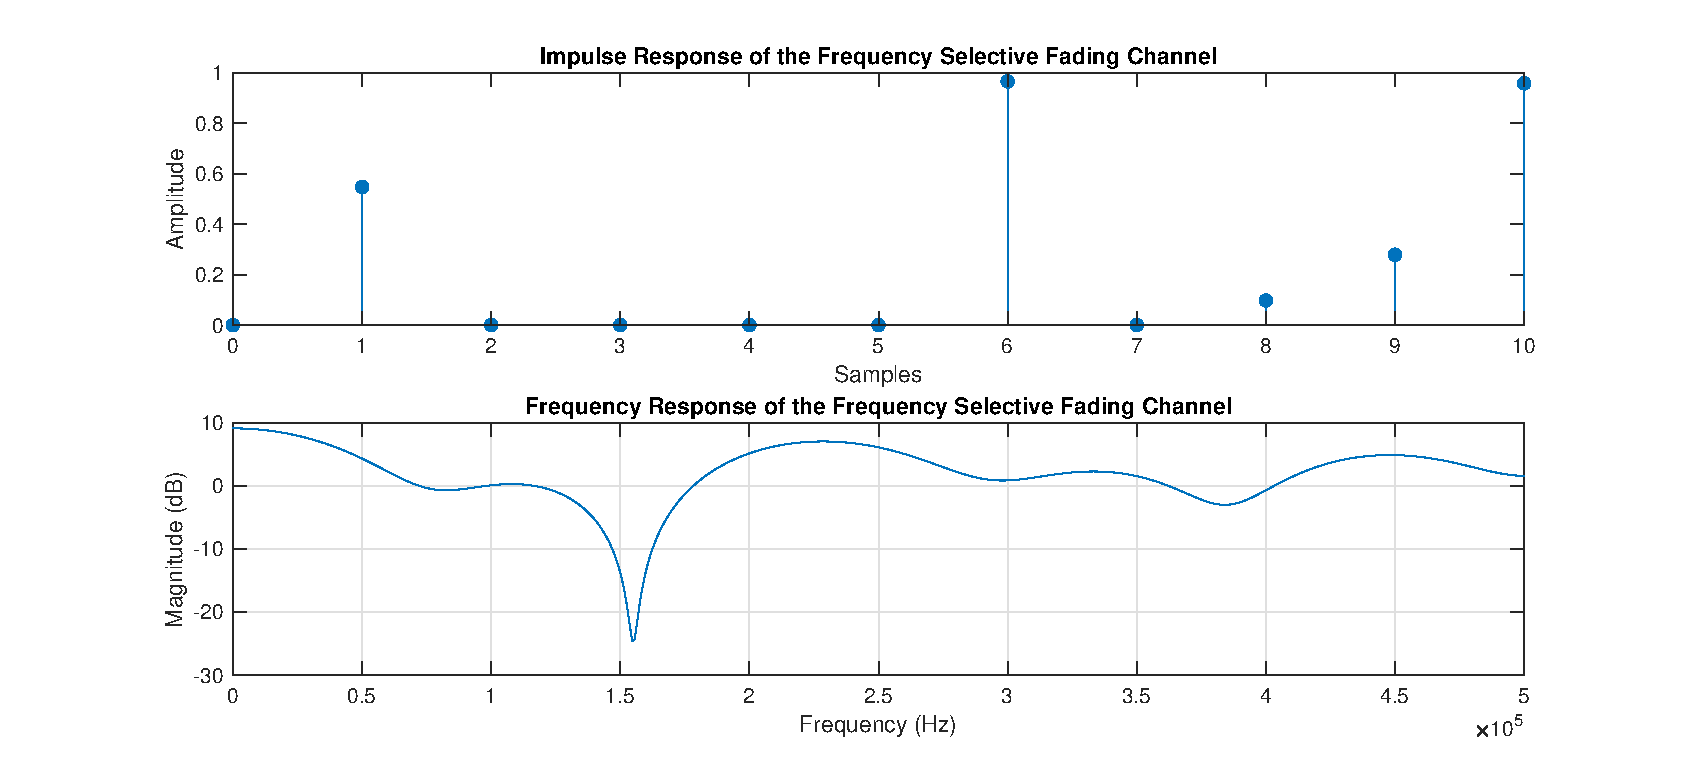
\includegraphics[width=\linewidth]{ffading.eps}
    \caption{Ten paths with different amplitudes.}
    \label{fig:ffading}
\end{figure}

\subsection{Peak to Average Power Ratio, Doppler Shift and Intercarrier Interference (ICI)}
We have explored many advantages of the OFDM system above and need to cover its weakness. Historically, the computation overhead of Discrete Fourier Transform (DFT) could be one but has been perfectly solved by Fast Fourier Transform (FFT). The high Peak to Average Power Ratio (PAPR) and sensitivity to Doppler Shift are two remaining issues.

The high PAPR is a common issue in the OFDM system. The OFDM system employs a large number of subcarriers in each OFDM symbol duration and has independent information symbols on each subcarrier. The independence means that the phases and amplitudes of the subcarriers can align at certain time instances, resulting high peak power. The high peak power requires the power amplifier to have a large dynamic range, which is expensive and inefficient. The high PAPR also causes the signal to be distorted by the power amplifier, which degrades the system performance. The quantitative analysis of PAPR issue is shown below. The PAPR is defined as
\begin{equation}
    \text{PAPR} = \frac{\max\abs{x_n}^2}{\E{\abs{x_n}^2}}, \quad n=0,1,\ldots,N-1.
\end{equation}
Since the subcarriers are orthogonal (independent), the central limit theorem can be applied on~\cref{eq:IFFT} and $x_n$ can be approximated as complex Gaussian random variables with zero mean and variance $\sigma^2$ when $N$ is sufficiently large (which is preferred in practice). Then the max PAPR can be approximated as
\begin{align}
    \max\abs{x_n}^2
    &= \sum_{i=0}^{N-1} \sigma^2 = N\sigma^2 \\
    \E{\abs{x_n}^2}
    &= \sum_{i=0}^{N-1} \bracks*{\frac{\sigma}{\sqrt{N}}}^2 = \sigma^2 \\
    \max\text{PAPR}
    &= N. \label{eq:papr}
\end{align}
The probability of PAPR exceeding certain threshold $P_0$ is
\begin{equation}
    \label{eq:papr_prob}
    \P{\text{PAPR}>P_0} = 1 - (1-e^{-P_0})^N.
\end{equation}
The~\cref{eq:papr_prob} states the PAPR will exceed certain threshold with high probability when $N$ is large. And the~\cref{eq:papr} states the PAPR can be as large as $N$. The high PAPR can be compensated by clipping the OFDM signal above some threshold, using spread spectrum to reduce the peak power, \etc. The~\cref{fig:PAPR} shows the PAPR of the OFDM system with different number of subcarriers.

\begin{figure}[!htbp]
    \centering
    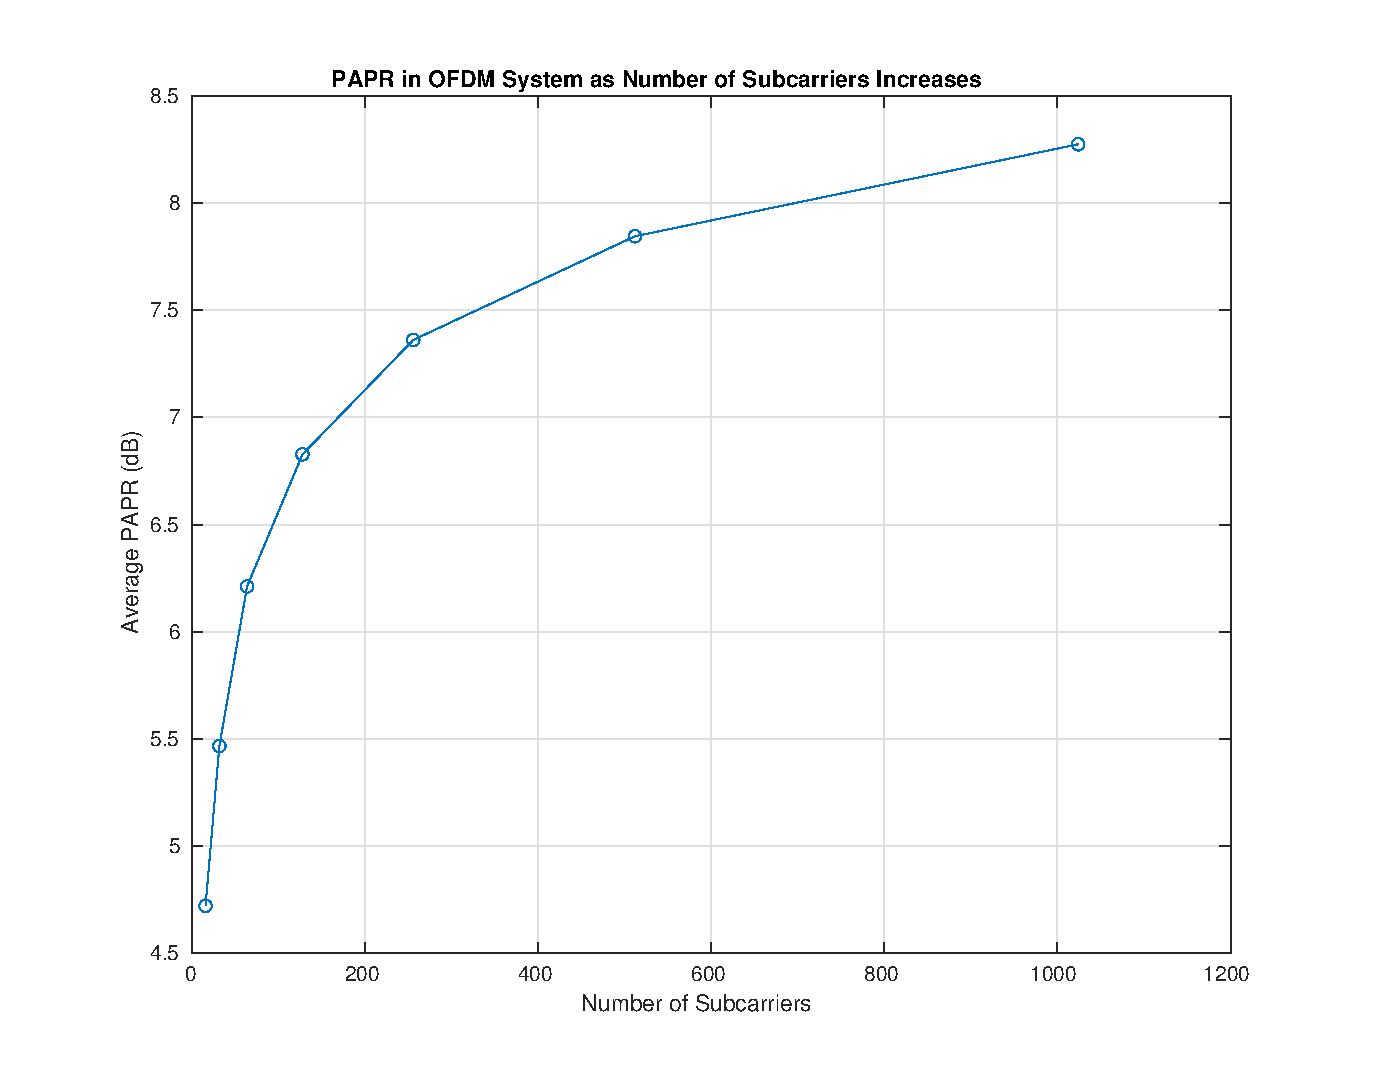
\includegraphics[width=\linewidth]{PAPR.eps}
    \caption{BPSK, Average of $5$ simulations for each number of subcarriers.}
    \label{fig:PAPR}
\end{figure}

Another issue is that OFDM is sensitive to Doppler Shift. The Doppler Shift in the channel will cause frequency shift in the received signal. This will reduce the SNR because the matched filter is designed to match the carrier frequency. The OFDM suffers more from the Doppler Shift because the OFDM system has a large bandwidth and the Doppler Shift can cause the subcarriers to shift out of the subcarrier spacing. This will cause the orthogonality of the subcarriers to be violated and the intercarrier interference (ICI) to be introduced. From the matrix analysis perspective, the $\Lambda$ in~\cref{eq:demod} will not be diagonal under the Doppler Shift. The Doppler Shift can be compensated in many ways.
\begin{enumerate}[(i)]
    \item Increase the subcarrier spacing to reduce the sensitivity to the Doppler Shift. But this will reduce the symbol rate and the system capacity.
    \item Use equalization to improve the SNR. However, equalization does not work well when the Doppler Shift is large. Besides, the equalization needs to know the channel transfer function, which is not always viable in the system or cannot be accurately estimated in the fast time-varying channel.
    \item Error Correction Coding (ECC) can be used to improve the system robustness. However, the ECC will introduce additional overhead and reduce the system capacity.
    \item New modulation schemes such as the Orthogonal Time Frequency Space (OTFS), which designs the waveform to be invariant to the Doppler Shift by using delay-Doppler domain signal representation. However, OTFS is not easy to be equalized as OFDM and the system complexity is higher than OFDM. The delay-Doppler domain channel estimation is also challenging.
\end{enumerate}

In conclusion, although OFDM system is able to overcome ISI and frequency-selective fading while maintain high symbol rate under complex channel condition, the maximum capacity is still bounded by the high PAPR and Doppler Shift. Overcoming these issues is the key to design the next generation wireless communication system.



\section{Synchronization and Pilot Symbols Aided Channel Estimation}
In the above content, the channel transfer function is an important component to help the OFDM system reach the optimal performance. The channel transfer function is obtained by channel estimation. A common approach is using the pilot symbols. In this section, we will discuss such a technique.



\section{Simulation Results}
We conduct experiments to illustrate the properties of the OFDM system. The experiment setup is as follows.
\begin{itemize}
    \item The experiment is done in MATLAB.
    \item The modulation scheme is 16-QAM.
    \item The OFDM system has 64 subcarriers.
    \item There are $10^5$ iterations. Each iteration has 3 OFDM symbols.
    \item The cyclic prefix is added in between OFDM symbols and its length is either 3 or 16.
    \item The Channel condition is either AWGN or Rayleigh fading. For the Rayleigh fading channel, the channel is set to have 5 taps with the delay spread being $[0, 3, 5, 6, 8]$ and the channel power being $[0, -8, -17, -21, -25]$.
    \item We evaluate the average Bit Error Rate (BER) vs.\. the EbN0 (dB) over iteration with EbN0 being $[0:5:30]$.
    \item The simulation result is shown in~\cref{fig:BER}.
\end{itemize}

\begin{figure}[!htbp]
    \centering
    \begin{subfigure}[t]{0.5\linewidth}
        \centering
        \caption{AWGN Channel with 3-tap CP}
        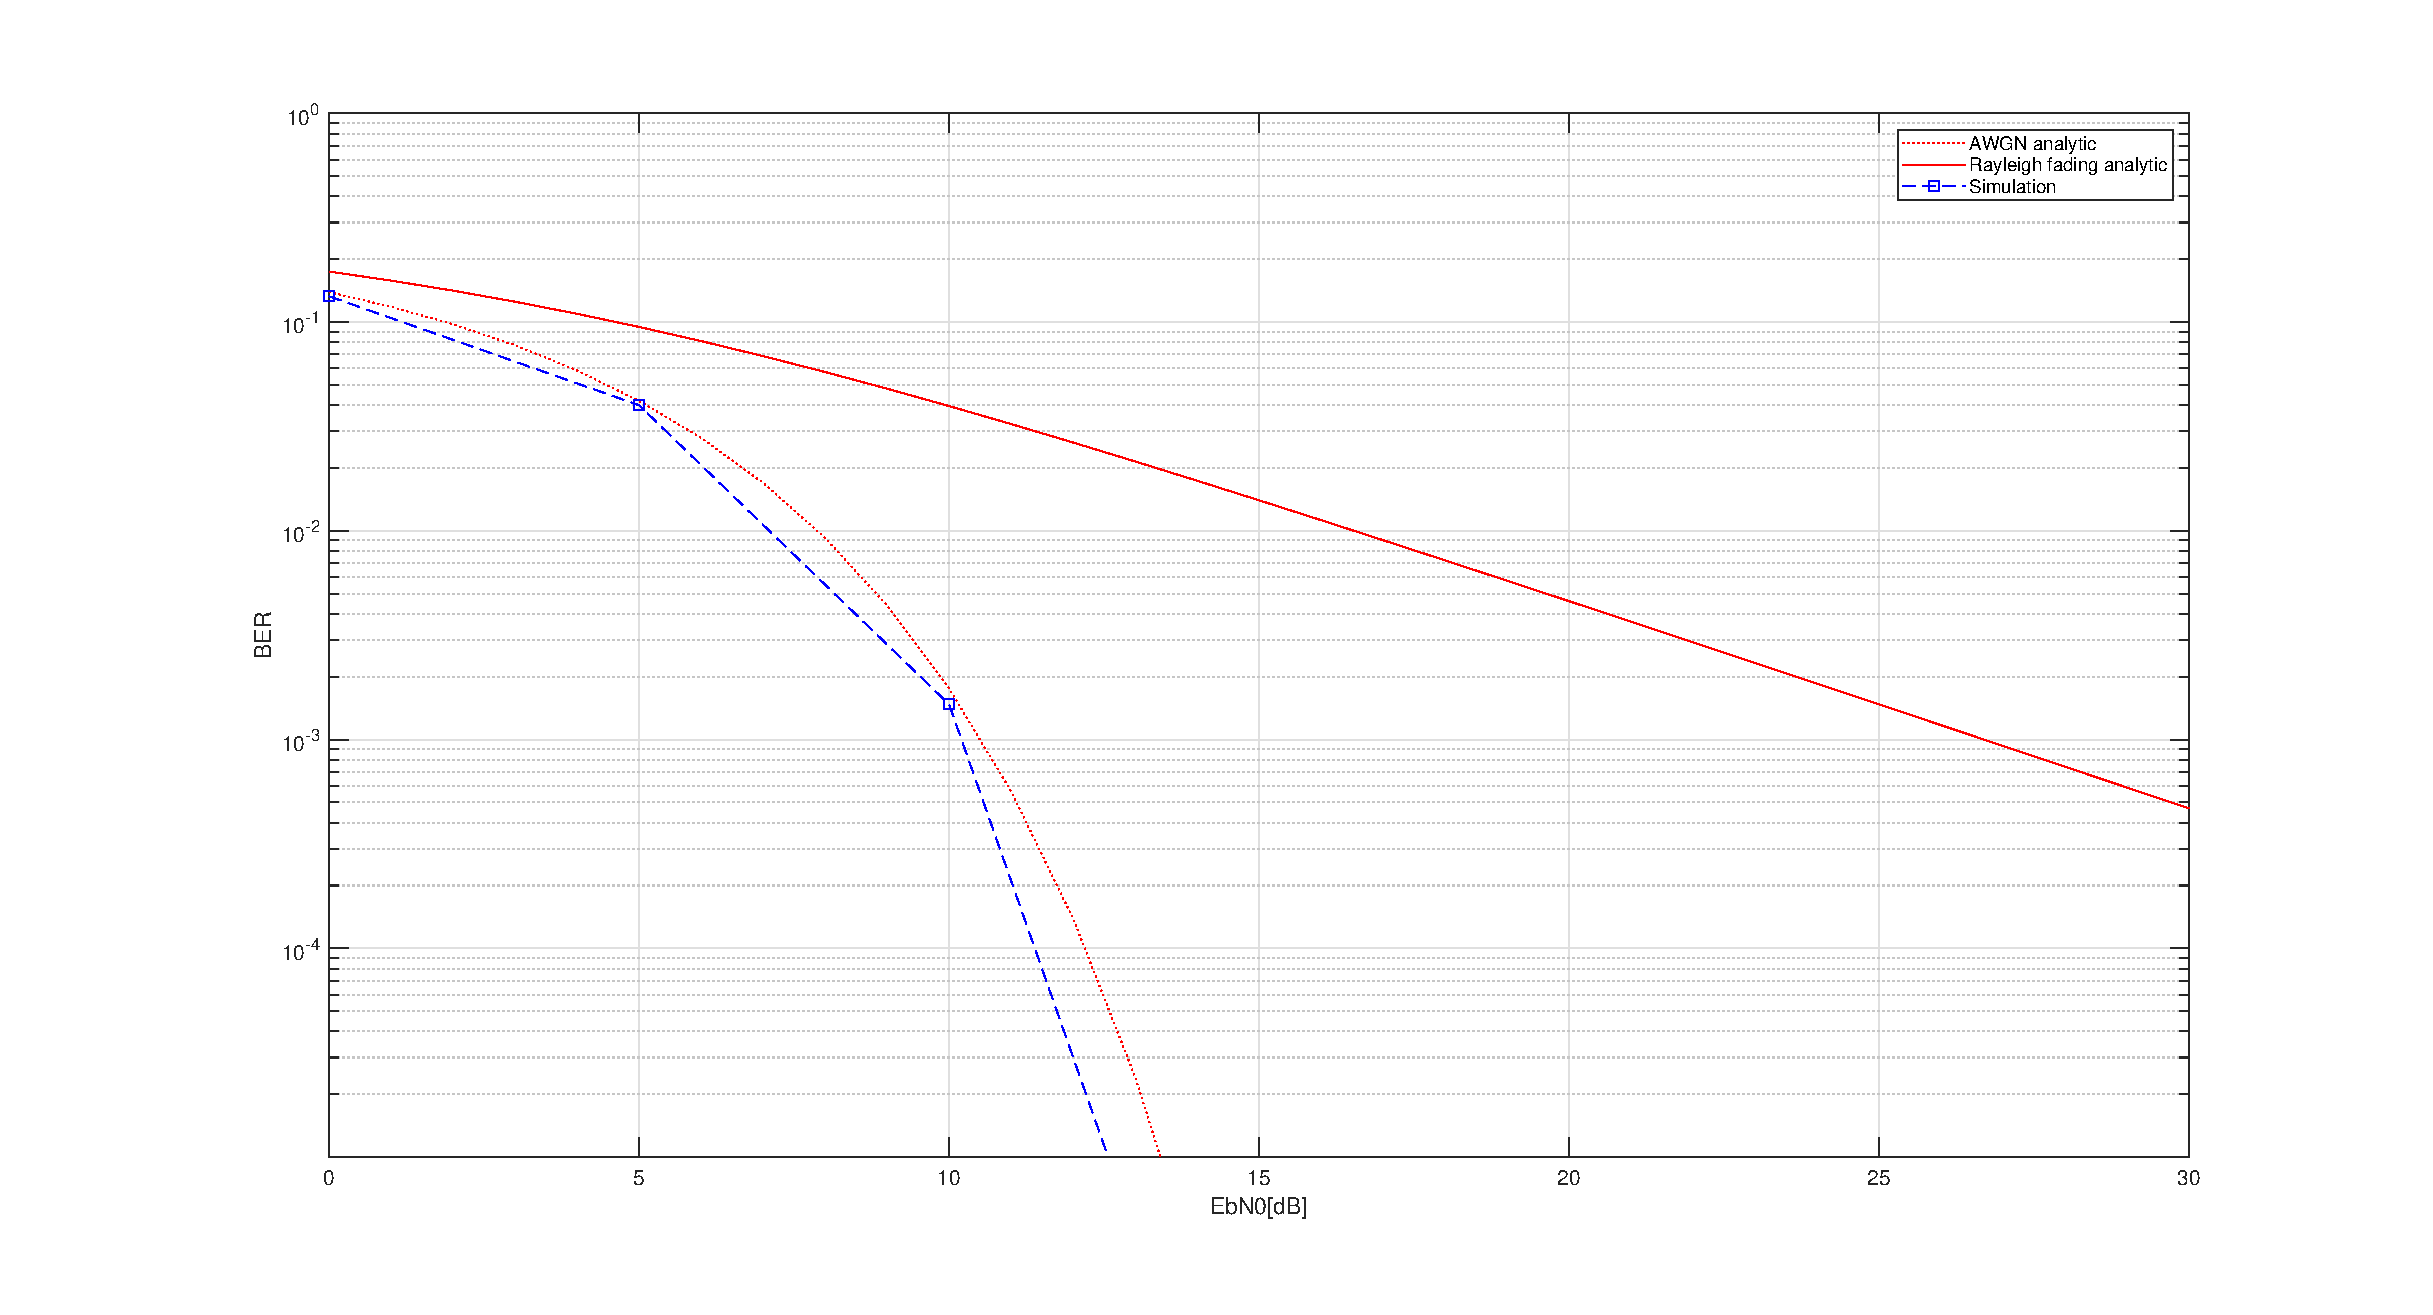
\includegraphics[width=\linewidth]{AWGN_3.eps}
        \label{fig:AWGN_3}
    \end{subfigure}%
    % ~
    \begin{subfigure}[t]{0.5\linewidth}
        \centering
        \caption{AWGN Channel with 16-tap CP}
        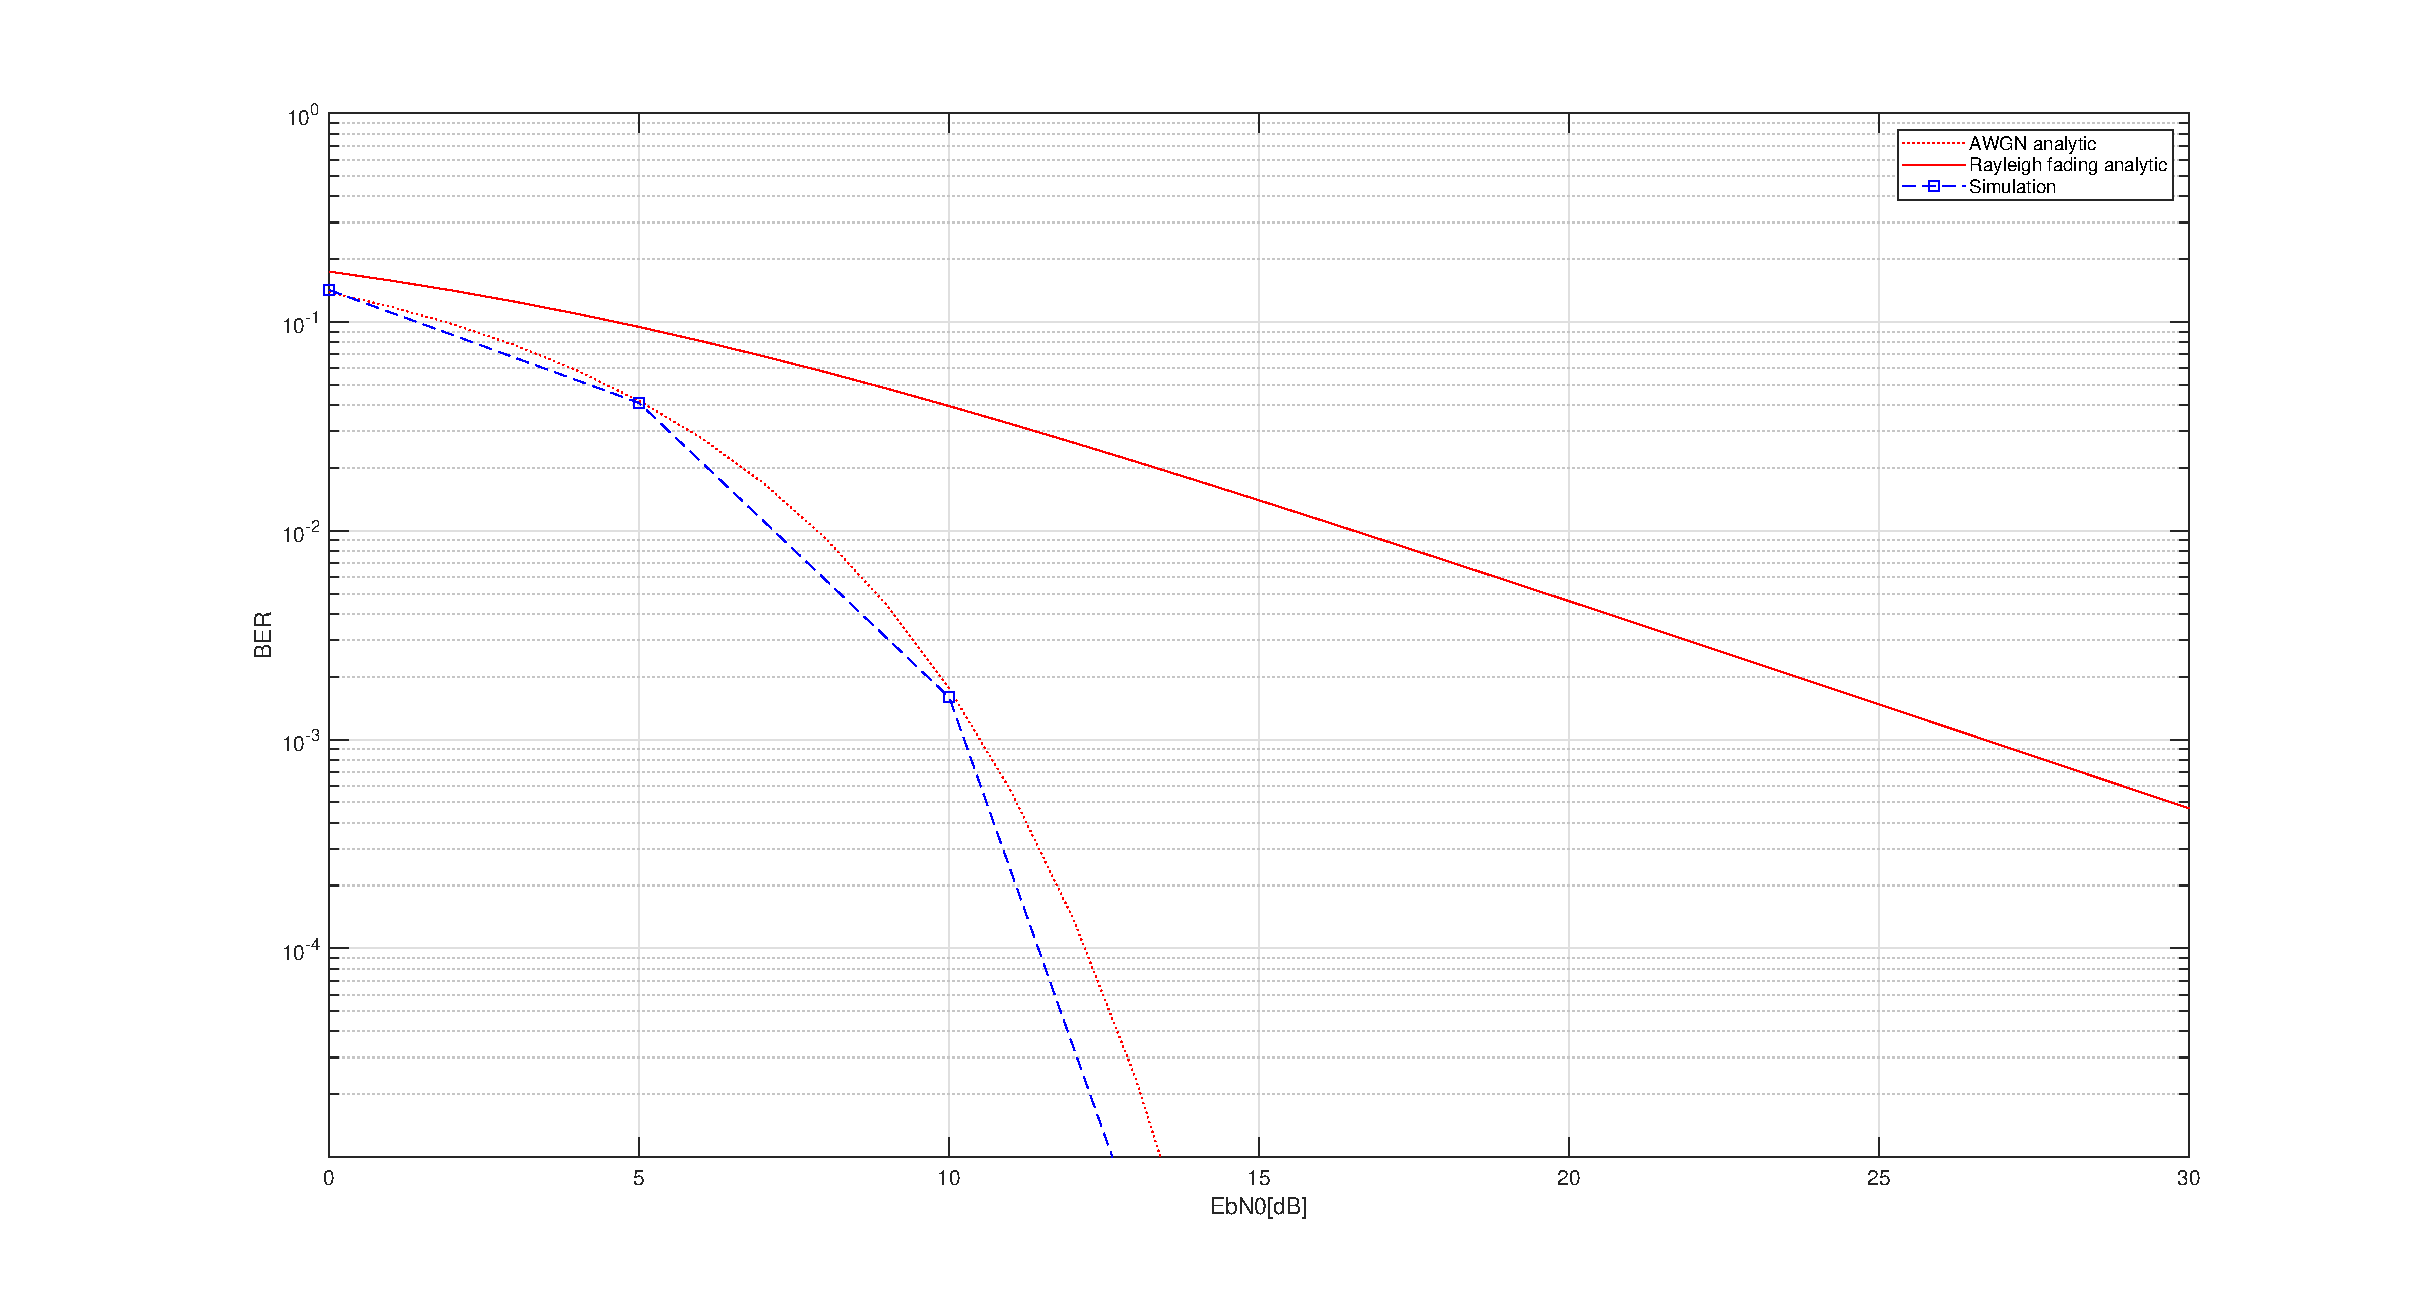
\includegraphics[width=\linewidth]{AWGN_16.eps}
        \label{fig:AWGN_16}
    \end{subfigure}%
    \\ %
    \begin{subfigure}[t]{0.5\linewidth}
        \centering
        \caption{Rayleigh Channel with 3-tap CP}
        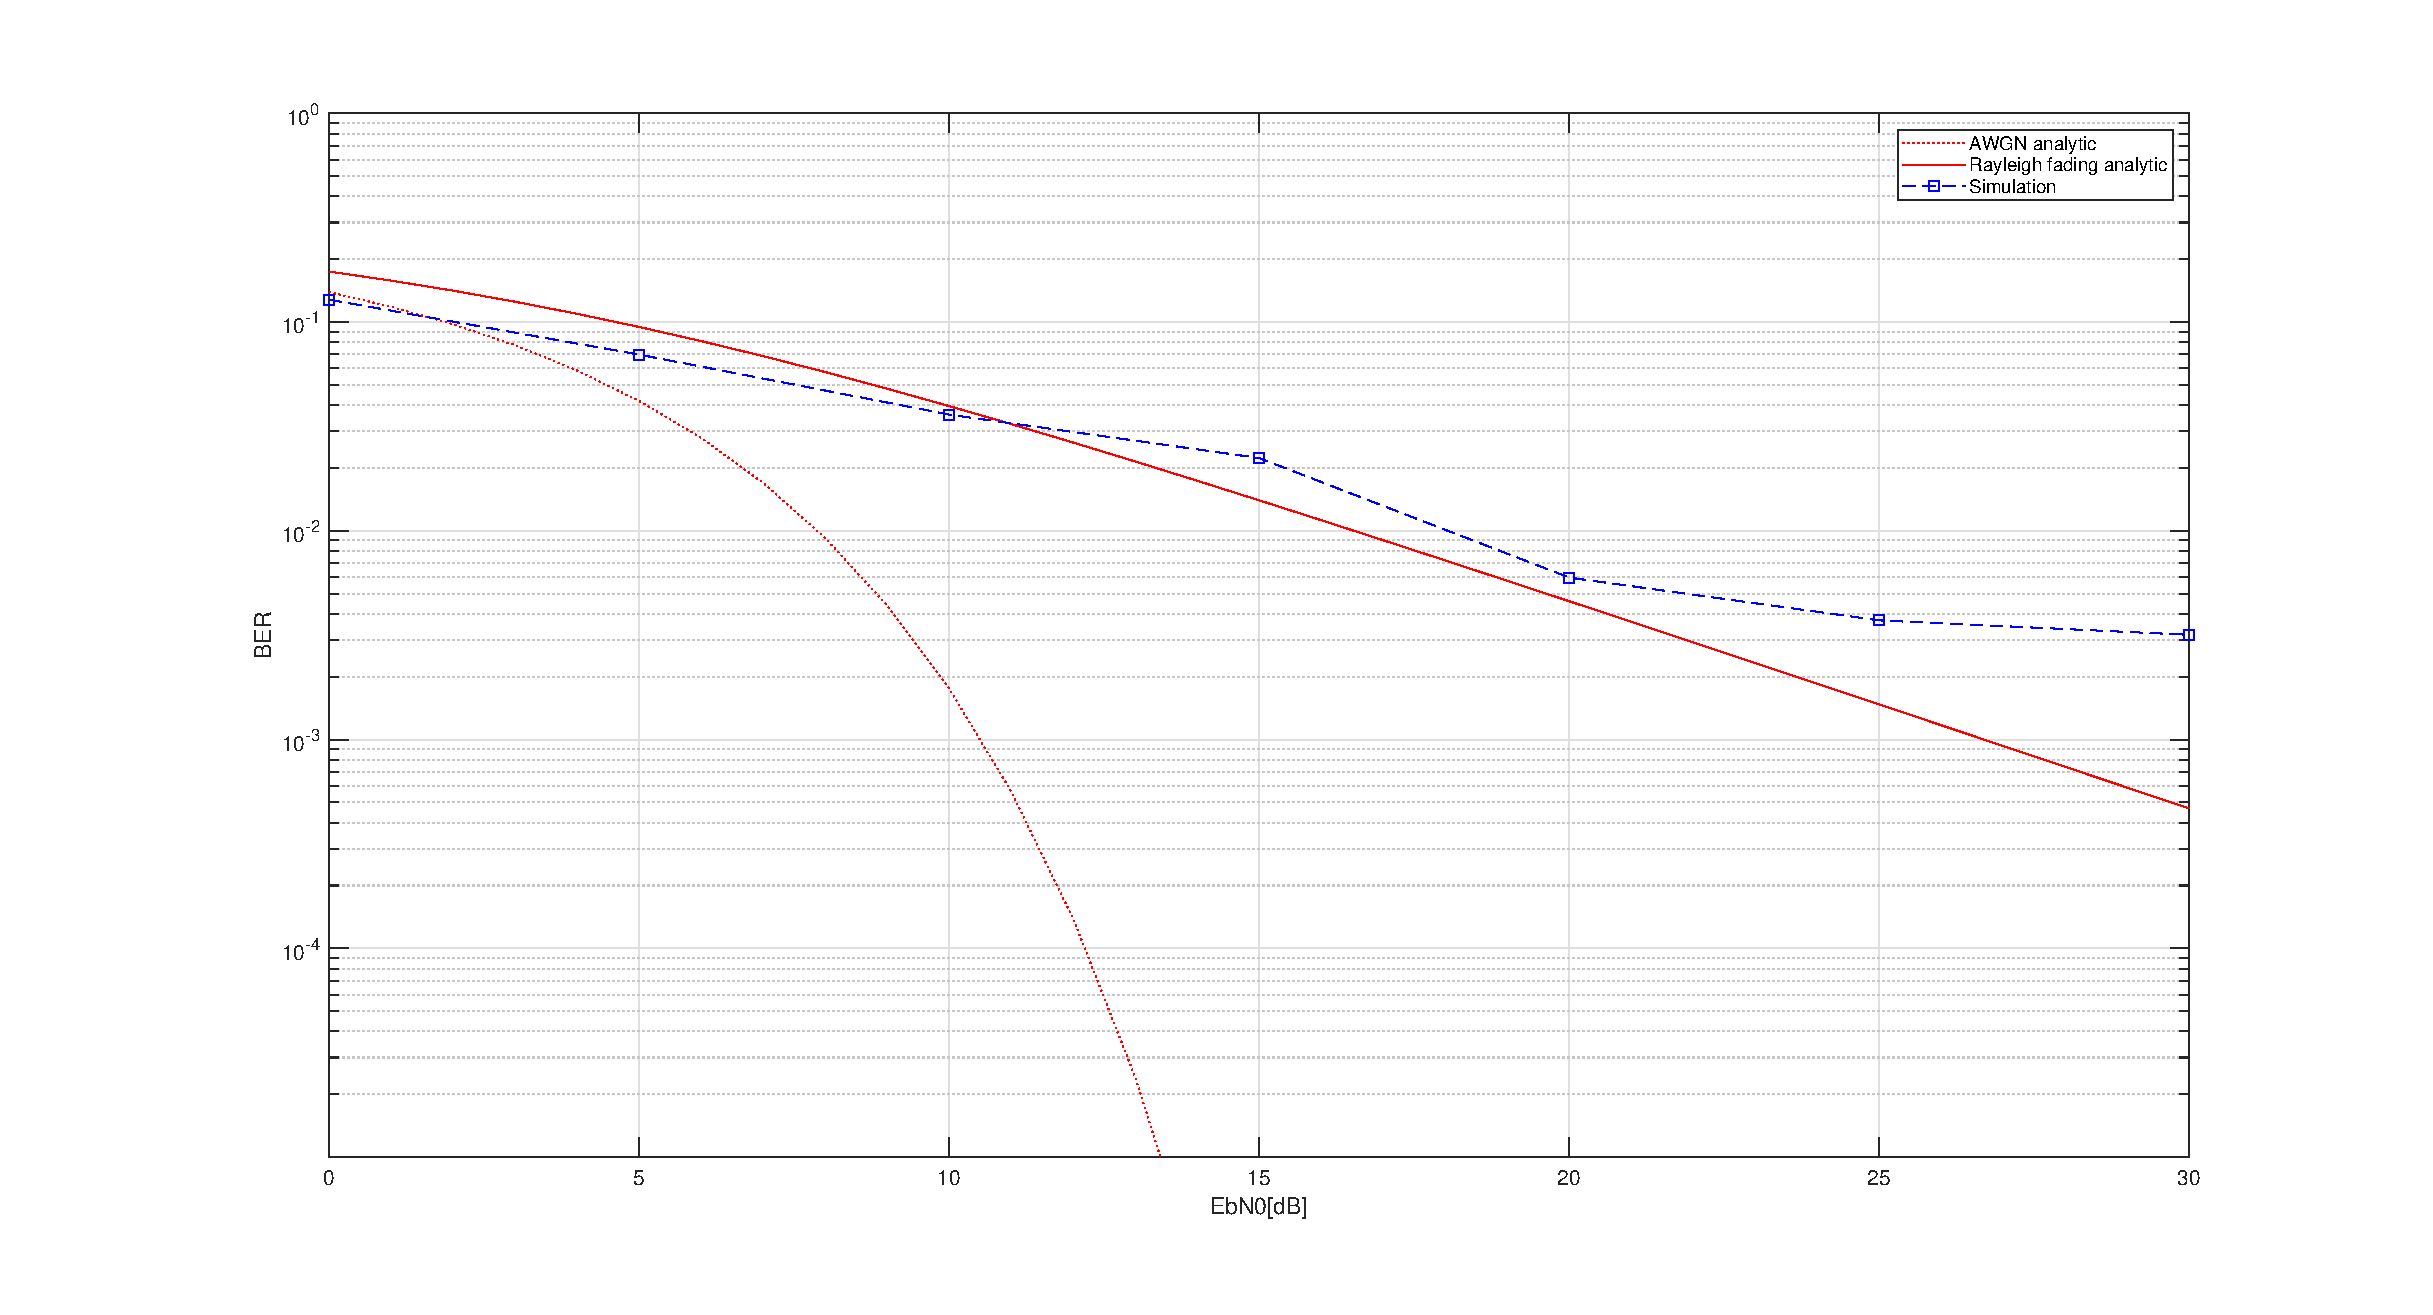
\includegraphics[width=\linewidth]{Rayleigh_3.eps}
        \label{fig:Rayleigh_3}
    \end{subfigure}%
    % ~
    \begin{subfigure}[t]{0.5\linewidth}
        \centering
        \caption{Rayleigh Channel with 16-tap CP}
        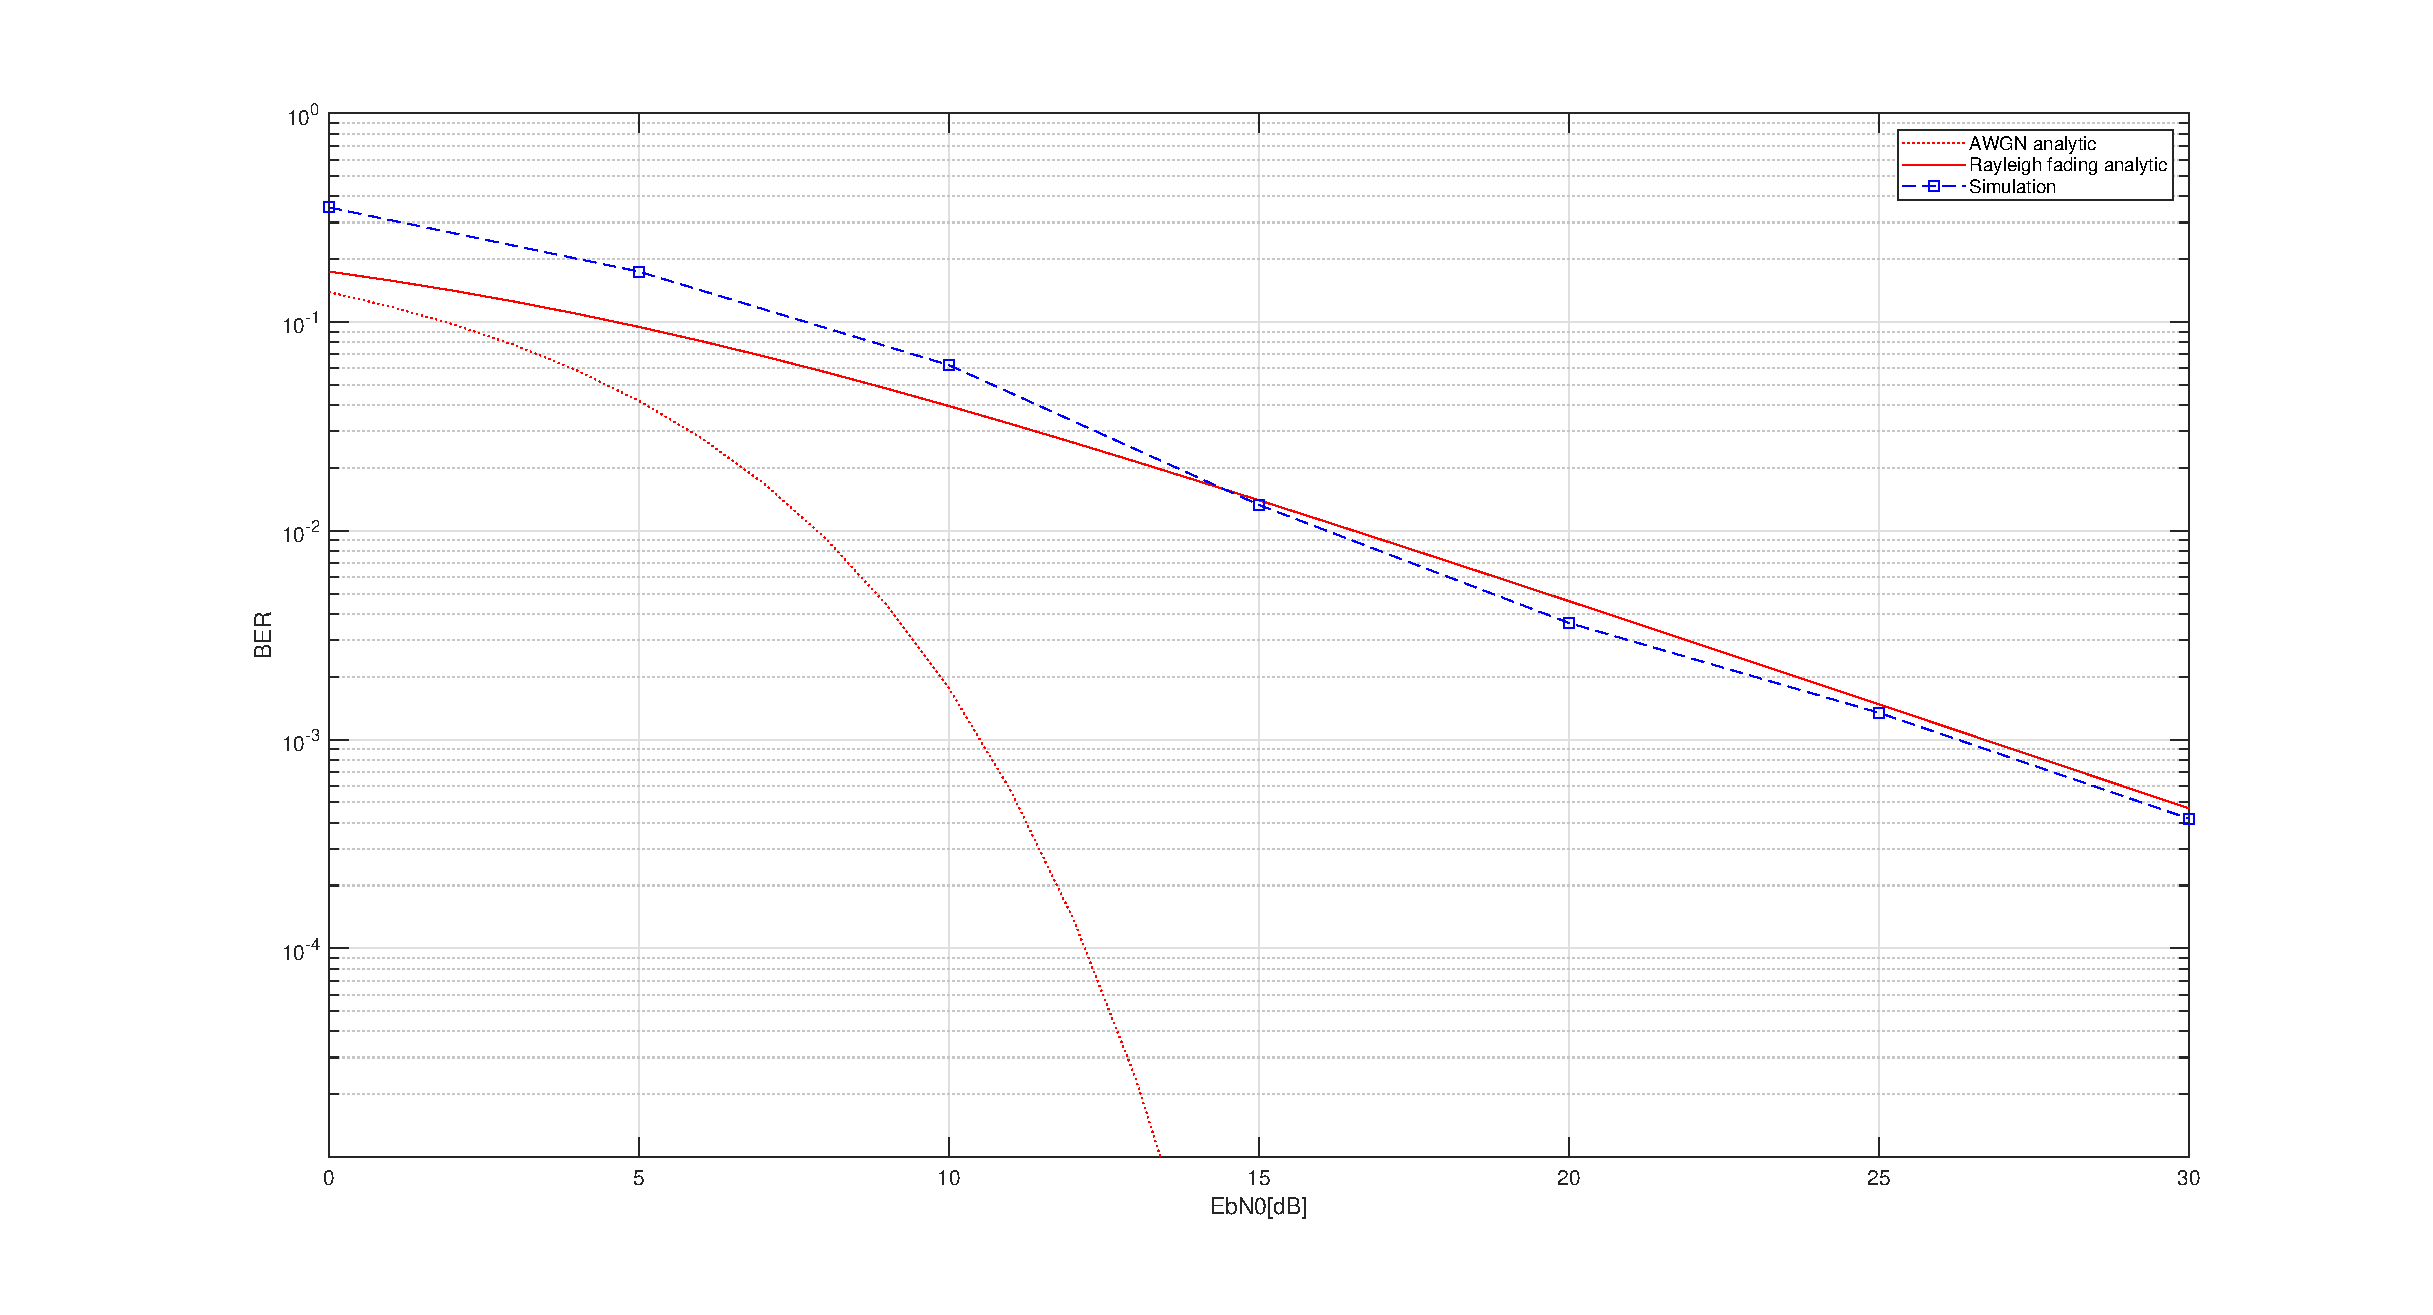
\includegraphics[width=\linewidth]{Rayleigh_16.eps}
        \label{fig:Rayleigh_16}
    \end{subfigure}%
    \caption{BER performance for OFDM system with 16-QAM. The~\cref{fig:AWGN_3,fig:AWGN_16} are for AWGN channel. The different CP length does not affect the simulation results since the flat fading has constant complex gain on the transmitted signal. The~\cref{fig:Rayleigh_3,fig:Rayleigh_16} are for Rayleigh fading channel with 5 taps. The simulation results show that the BER exceeds the analytical result if the CP length is shorter than the delay taps, while the BER will be closed to the analytical result if the CP length is longer than the delay taps. The result implies that the OFDM system is only subject to flat fading as long as the CP length is longer than the channel delay spread.}
    \label{fig:BER}
\end{figure}

\section{Conclusion}
In this report, we introduce the OFDM modulation and demodulation process, discuss its mathematical properties, and evaluate its performance with simulations. We show that the OFDM system is robust to frequency-selective fading and intersymbol interference. The simulation results demonstrate that the OFDM system is only subject to flat fading as long as the cyclic prefix length is longer than the channel delay spread. The OFDM system is widely used in modern wireless communications due to its high symbol rates and robustness to channel impairments.

\clearpage
\printbibliography

\end{document}